% Author: Pavol Loffay
% Project: Master thesis - Hawkular alrt prediction
% Date 20.2.2015

\chapter{Introduction} 
Alert prediction is very important because it can predict states of a system in
advance.  

\section{Context}
Implementation part of the master thesis developer as part of the project
Hawkular, therefore it affects application architecture, used technologies and
also used methods of forecasting.

Project Hawkular is open source monitoring and management platform mainly
developed by Red Hat. This application is designed to monitor Java middleware 
like Wildfly, Apache Tomcat. For instance it can monitor heap usage, web
sessions, used data sources \dots

\section{Goals}
The main goal of the application is to provide users with reliable predictions
of alerts for the set of collected metrics. Displaying of forecast is also
available in the user interface. This feature can help system administrators
help in advance to react events like running out of memory.

\chapter{Time Series Analysis}

\chapter{Design and Implementation}
\section{Architecture}
\scalebox{0.5}{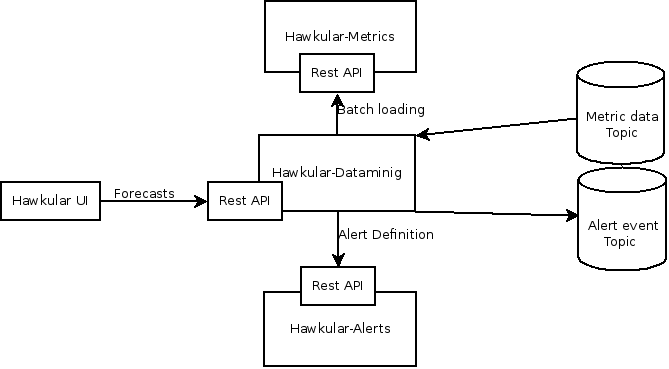
\includegraphics{img/architecture.png}}

\chapter{Conclusion}
\cite{rfc_owamp} %TODO remove

